\subsection{Timer Modules}
\label{sec:timers}
The HPS includes several hardware timer modules that can be used to keep track of time intervals.
The ARM A9 MPCore includes one {\it private} timer module for each A9 core, and the
HPS provides four other timer modules that can be used by either A9 core. The timers are 
described in more detail below.

\subsubsection{ARM* A9* MPCore* Timers}
\label{sec:ARM_timers}
Figure~\ref{fig:MPCORE_timer} shows the registers in the programmer's interface for each
A9 core private timer. These registers have the base address {\sf 0xFFFEC600}, as shown in
the figure, and can be read or written using word accesses. To use the timer, 
it is necessary to first write an
initial count value into the {\it Load} register. The timer can then be started by
setting the enable bit $E$ in the {\it Control} register to 1, and it can be stopped by
setting $E$ back to 0.  Once enabled the timer decrements its count value until reaching 0.
When it reaches 0, the timer sets the {\it F} bit in the {\it Interrupt status} register. 
The {\it F} bit can be checked by software using polled-I/O to determine when the timer
period has expired.  The {\it F} bit can be reset to 0 by writing a 1 into it. 
Also, if bit~{\it I} in the {\it Control} register is set to 1,
then a processor interrupt can be generated when the timer reaches 0.  Using 
interrupts with the timer is discussed in Section~\ref{sec:exceptions}.

When it reaches 0, the timer will stop if the auto bit ({\it A}) in the control register
is set to 0.  But if bit {\it A} is set to 1, then the timer will automatically reload the 
value in the {\it Load} register and continue decrementing. The current value of the timer is
available to software in the {\it Counter} register shown in Figure~\ref{fig:MPCORE_timer}.
The timer uses a clock frequency of 200 MHz. The {\it Prescaler} field in the {\it
Control} register can be used to slow down the counting rate, as follows. The timer decrements 
each {\it Prescaler} $+1$ clock cycle. Therefore, if {\it Prescaler} $=0$, then the
timer decrements every clock cycle, if {\it Prescaler} $=1$, the timer
decrements every second clock cycle, and so on.

\begin{figure}[h!]
   \begin{center}
       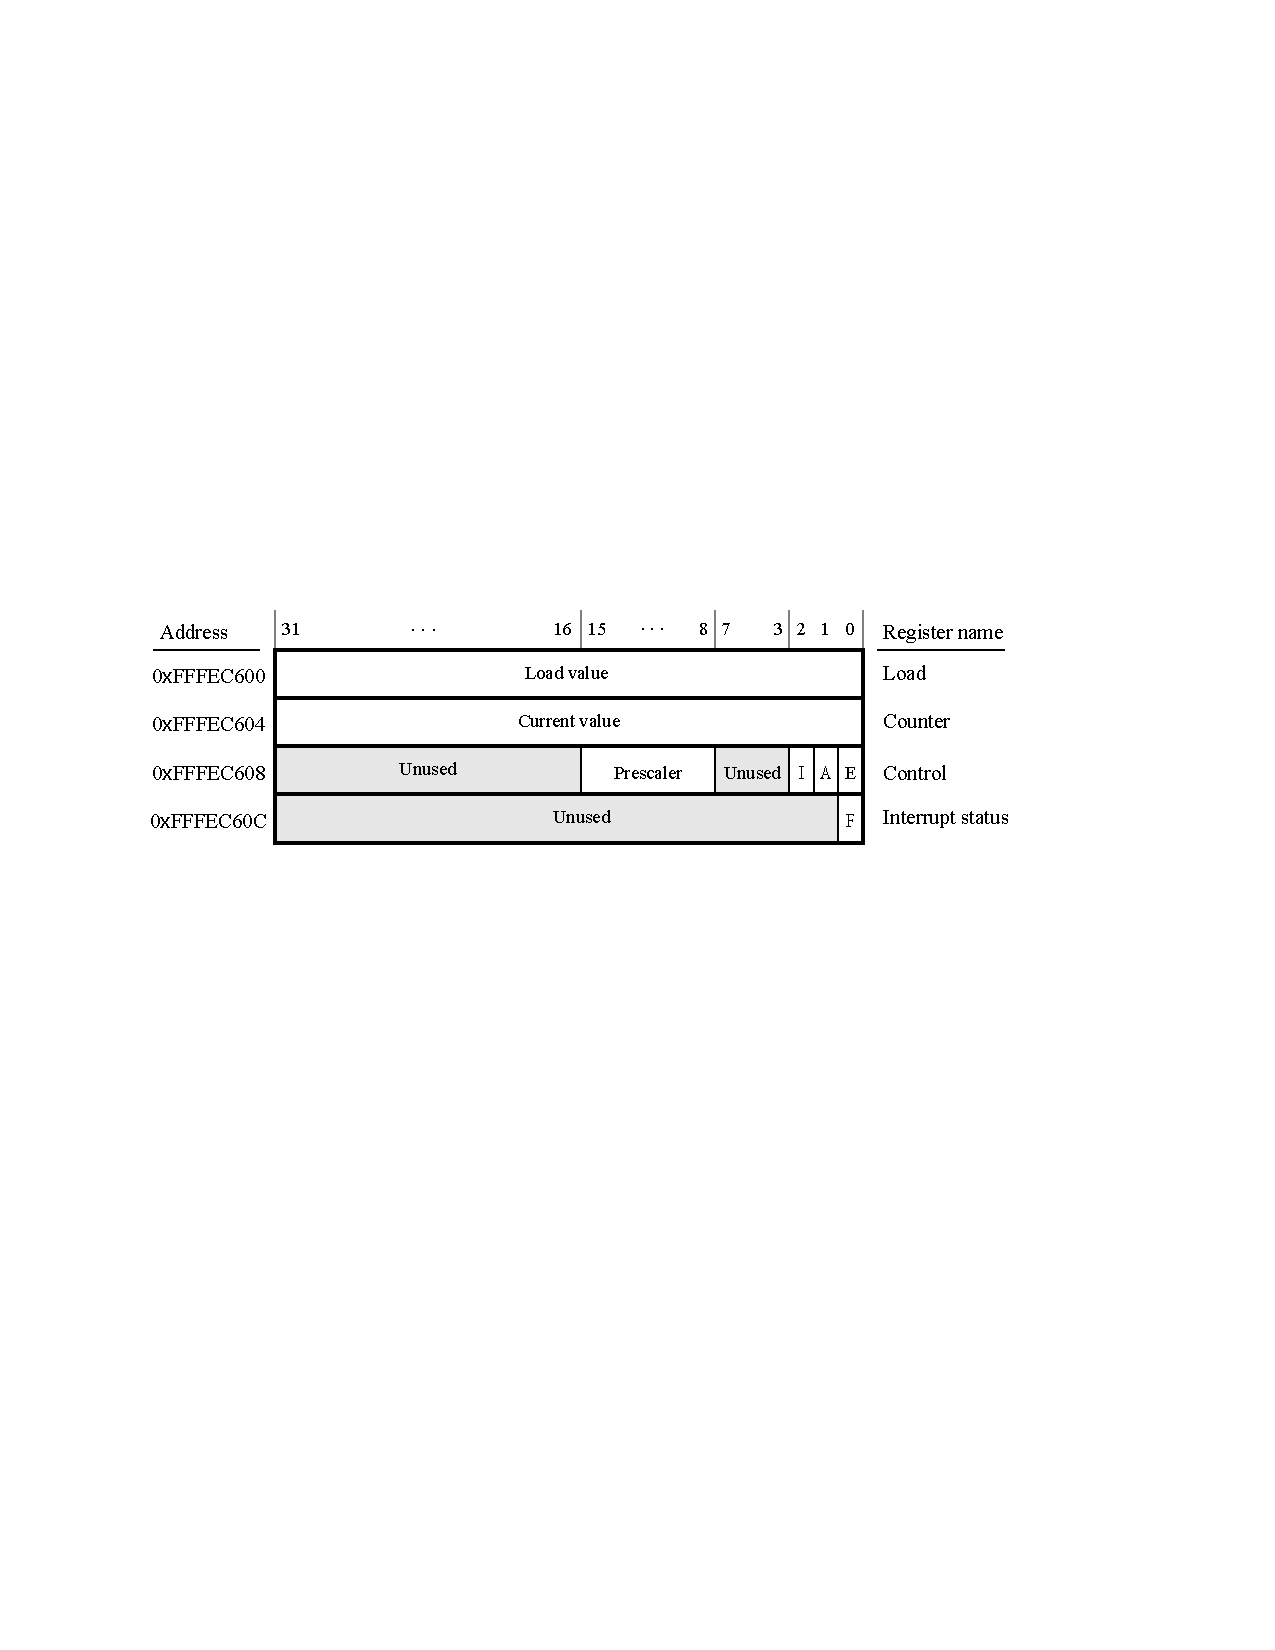
\includegraphics{../../../common/figs/HPS_MPCORE_Timer.pdf}
   \end{center}
   \caption{ARM A9 private timer port.}
	\label{fig:MPCORE_timer}
\end{figure}

\subsubsection{HPS Timers}
\label{sec:HPS_timers}
Figure~\ref{fig:HPS_timer} shows the registers in the programmer's interface for one of 
the HPS timers.  These registers have the base address {\sf 0xFFC08000}, as shown in
the figure, and can be read or written using word accesses. To configure the timer, 
it is necessary to ensure that it is stopped by setting the enable bit $E$ 
in the {\it Control} register to 0. A starting count value for the timer can then be written into
the {\it Load} register. To instruct the timer to use the specified starting count value, the
{\it M} in the {\it Control} register should be set to 1, and the timer can be started by 
setting $E = 1$. The timer counts down to 0, and then sets both bit $F$ in the 
{\it End-of-interrupt} register and bit {\it S} in the {\it Interrupt status} register to 1. 
Software can poll the value of $S$ to determine when the timer period has expired. 
The {\it S} bit, and the {\it F} bit can be reset to 0 by reading the contents of 
the {\it End-of-Interrupt} register.  Also, if bit $I$, the interrupt mask bit, in 
the {\it Control} register is set to 0, then an interrupt can be generated when 
the timer reaches 0 (note that bit {\it I} in the ARM A9 private timer shown in 
Figure~\ref{fig:MPCORE_timer} has the opposite polarity). The use of interrupts with the
timer is discussed in Section~\ref{sec:exceptions}.

The current value of the timer is available to software in the {\it Counter} register shown in 
Figure~\ref{fig:HPS_timer}.  The timer uses a clock frequency of 100 MHz. 

There are three other identical timers in the HPS, with the following base
addresses: {\sf 0xFFC09000}, {\sf 0xFFD00000}, and {\sf 0xFFD01000}. The first of these
timers uses a 100 MHz clock, and the last two timers use a 25 MHz clock.

We should mention that other timer modules also exist in the HPS. The ARM A9 MPCore has
a {\it global} timer that is shared by both A9 cores, as well as a {\it watchdog} timer
for each processor. Also, the HPS has two additional watchdog timers. Documentation about
the global timer and watchdog timers is available in the {\it ARM Cortex A9 MPCore
Technical Reference Manual}, and in the {\it Cyclone V Hard Processor System
Technical Reference Manual}.

\begin{figure}[h]
   \begin{center}
       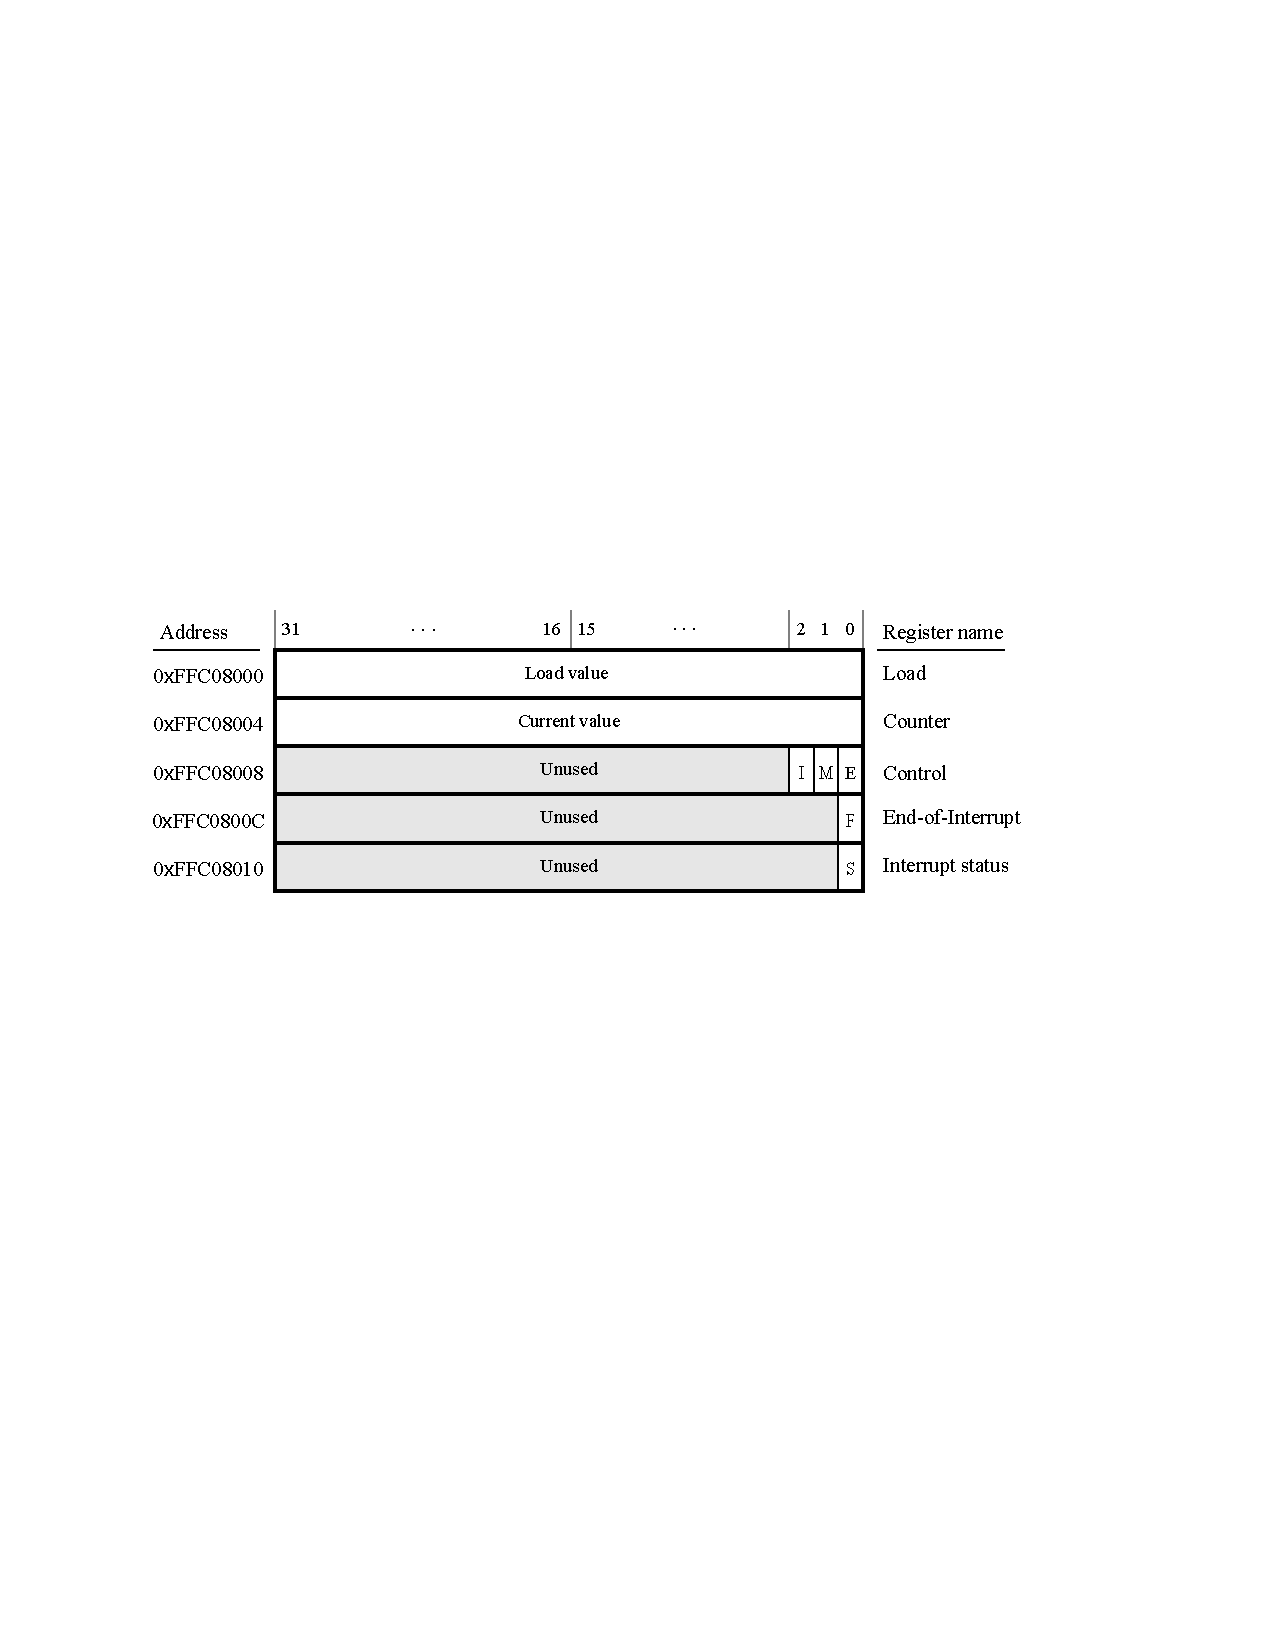
\includegraphics{../../../common/figs/HPS_Timer.pdf}
   \end{center}
   \caption{HPS timer port.}
	\label{fig:HPS_timer}
\end{figure}

\subsubsection{Using a Timer with Assembly Language Code}
\label{sec:ARM_assembly}
An example of ARM A9 assembly language code is included in the Appendix in Listing~\ref{lst:timer_s}. The code 
configures the private timer for the A9 core so that it produces one-second timeouts. An
infinite loop is used to flash the green light connected to GPIO1, discussed
in Section \ref{sec:hps_gpio1}. The light is turned on for one second, then off, and so on.

An example of C code is also included in Listing~\ref{lst:timer_C}. This code performs the same actions 
as the assembly language program in Listing~\ref{lst:timer_s}---it flashes on/off the green 
light connected to GPIO1 at one-second intervals.

The source code files shown in Listings~\ref{lst:timer_C} and~\ref{lst:timer_s}
are distributed as part of the  
\productNameMed{}. The files can be found under the heading {\it sample programs}, 
and are identified by the name {\it Timer Lights}.


